%!TEX root = ../Chapter4.tex
\section{A Gamified Algorithm}\label{sec:lgc.game}

The first attempt using Bayesian machinery does not end up with a satisfying output. In this section, we turn our thoughts to another idea and take inspiration from the \emph{zero-sum game} (see e.g.~\citealt{degenne2019pure}). We describe \gls{lg}, detailed in Algorithm~\ref{alg:lg}. As noted in the seminal work of \citet{chernoff1959}, the complexity $\Tstar(\btheta)^{-1}$ is the value of a fictitious zero-sum game between the learner choosing an optimal proportion of allocation of pulls $\bomega$ and a second player, the nature, that tries to fool the agent by responding with the most confusing alternative $\btheta'$ leading to an incorrect answer. \gls{lg} is an asymptotically optimal algorithm for linear bandits \gls{bai}. Note that the present algorithm is asymptotically optimal for the general pure exploration game, which is however not the main focus of this thesis. Lecturers can refer to~\cite{degenne2020game} for more details.

In this section, we make the following extra assumption.
\begin{assumption}\label{ass:lgc.bounded_parameter}
\begin{leftbar}[assumptionbar]
We assume that $\exists M>0$, s.t. $\forall \btheta\in\Theta$, $\normm{\btheta} \leq M$, where $\normm{\btheta}$ denotes the Euclidean norm of the vector $\btheta$. 
\end{leftbar}
\end{assumption}

%The full analysis of the algorithm is omitted as well as a convexified version \LGC{} -- also asymptotically optimal itself -- as they are not the main focus of this thesis. Lecturers can refer to~\cite{degenne2020game} for the complete proofs.


% , i.e for $i\in\cI$ and $w\in\interior{\Sigma_A}$ in the interior of the probability simplex of dimension $A-1$, find $\lambda^i$ such that
% \[
% \lambda^i \in \argmin_{\lambda\neg i}\normm{\theta - \lambda }_{V_{w}}\,.
% \]


%Note that in the proof of Theorem~\ref{thm:sample_complexity} we only use two times the boundedness assumption, first in the definition of the threshold $\beta(t,\delta)$ (see Theorem~\ref{th:confidence_beta}) to handle the bias induced by the regularization. Second, since the regret of AdaHedge is proportional to the maximum of the upper confidence bounds $U_s^{i,a}$, we need to ensure that they are bounded.

% And there exists pathological pure exploration problems where even the quantity uppper bounded by $U_s^{i,a}$, namely $\normm{\theta-\lambda}_{aa^\top}^2$ where $\lambda\in\argmin_{\lambda'\in\neg i}\normm{\theta -\lambda}$ is unbounded\todo{I don't understand what this means.}. See for example Appendix~G.3 by \citet{menard2019lma}.

\subsection{Notation}

In this section, besides the usual learner, we include an extra fictive player -- the nature -- and we thus introduce some specific notation of counts for this section.

At each round $n$ the algorithm to be presented will play an arm $\hbx_n$ and choose (fictitiously) an answer $i_n\in\cI$. We denote by $T_n^{\bx,i} \eqdef\sum_{t=1}^n \ind_{\{(\hbx_n,i_n)=(\bx,i)\}}$ the number of times the pair $(\bx,i)\in\cX\times\cI$ is chosen up to and including time $n$, and by $T_n^\bx =\sum_{i\in\cI} T_n^{\bx,i}$ and $T_n^i =\sum_{\bx\in\cX} T_n^{\bx,i}$ the partial sums\footnote{Note that if $i$ is the index of arm $\bx$, then $T_n^\bx$ is simply $T_{n,i}$ as defined in~\eqref{eq:mab.pulls}.}. The vectors of counts at time $n$ is denoted by $\bT_n \eqdef (T_n^\bx)_{\bx\in\cX}$
and when it is clear from the context we will also denote by $\bT_n^{\bx} = (T_n^{\bx,i})_{i\in\cI}$ and $\bT_n^i = (T_n^{\bx,i})_{\bx\in\cX}$ the vectors of partial counts. Recall that in the case of \gls{bai}, $\cX=\cI$.

%\paragraph{Regularized least square estimator.} We fix a regularization parameter $\eta > 0$. The regularized least square estimator for the parameter $\theta\in \mathcal M$ at time $t$ is
%\[
%\htheta_{t} = (V_{N_t} + \eta I_d)^{-1} \sum_{s=1}^t Y_s a_s\,,
%\]
%where $I_d$ is the identity matrix. By convention $\htheta_0 = 0$.


\subsection{The \LG{} algorithm}

The pseudo-code of \gls{lg} is provided in Algorithm~\ref{alg:lg}. We explain how it works in detail in the next.

\begin{algorithm}[ht]
\centering
\caption{Algorithm of \LG{}}
\label{alg:lg}
\begin{algorithmic}[1]
    \State {\bfseries Input:} Learners for each answer $(\cL^i_\bomega)_{i\in\cI}$, threshold $d$
    \For{n = 1 \ldots}
        \State \textit{// Stopping rule}
        \If{{$\max_{i\in\cI}\inf_{\btheta'\in\neg i} \frac{1}{2}\normm{\hbtheta_{n-1}^\lambda-\btheta'}^2_{\bLambda_{\bT_{n-1}}}\geq d_{n-1,\delta}$}}
            \State \text{Stop} 
            \State {\bfseries Return} $J_n = \Istar(\hbtheta_{n-1}^\lambda)$
        \EndIf
        \State \textit{// Empirical best guess}
        \State $i_n = \Istar(\hbtheta_{n-1}^\lambda)$
        \State \textit{// Learner plays first}
        \State \text{Get} $\bomega_n$ \text{from} $\cL^{i_n}_\bomega$
        \State \text{Update} $\bW_n=\bW_{n-1}+\bomega_n$
        \State \textit{// Best response of the nature}
        \State $\btheta_n^{i_n} \in \argmin_{\btheta'\in\neg i_n}\normm{\hbtheta_{n-1}^\lambda-\btheta'}^2_{\bLambda_{\bomega_n}}$
        \State \textit{// Feed optimistic gains}
        \State \text{Feed learner} $\cL_\bomega^{i_n}$ \texttt{with} $g_{n}(\bomega) = \sum_{\bx\in\cX}\omega_\bx U_n^{\bx,i_n}/2$
        \State \textit{// Track the weights}
        \State \text{Pull} $\hbx_n \in \argmin_{\bx\in \cX} T_{n-1}^{\bx} - W_{n,\bx}$
   \EndFor
\end{algorithmic}
\end{algorithm}

% \begin{algorithm}[tb]
% \centering
% \caption{\LGC}
% \label{alg:lgc}
% \begin{algorithmic}[1]
%     \State {\bfseries Input:} Agent learner $\cL_{\tw}$, threshold $\beta(\cdot,\delta)$
%     \For{t = 1 \ldots}
%         \State \textit{// Stopping rule}
%         \If{ {\small $\max_{i\in \cI} \inf_{\lambda\in\neg i} \frac{1}{2}\normm{\htheta_{t-1}-\lambda}^2_{V_{N_{t-1}}}\geq \beta(t-1,\delta)$}}
%             \State {\bfseries stop} and {\bfseries return} $\hi = \istar(\hat{\theta}_{t-1})$. 
%         \EndIf
%         \State \textit{// Agent plays first}
%         \State \texttt{get} $\tw_{t}$ \texttt{from} $\cL_{\tw}$ 
%         \State \texttt{update} $\tW_{t}=\tW_{t-1}+\tw_{t}$
%         \State \textit{// Best response for the nature}
%         \State $\forall i\in\cI$, $\tlambda^i_{t} \in \argmin_{\lambda\in\neg i}\normm{\htheta_{t-1}-\lambda}^2_{V_{\tw^i_{t}}}$
%         \State \textit{// Feed optimistic gains}
%         \State \texttt{feed learner} $\cL_{\tw}$ \texttt{with} {$g_{t}(\tw) =\sum_{(a,i)\in\cA\times\cI} \tw^{a,i} U_t^{a,i}/2$}
%         \State \textit{// Track the weights}
%         \State \texttt{pull} $(a_{t},i_{t})\in \argmin_{(a,i)\in \mathcal A \times \mathcal I} N_{t-1}^{a,i} - \tW_{t}^{a,i}$
%     \EndFor
% \end{algorithmic}
% \end{algorithm}

\paragraph{Stopping rule and decision rule.}
We follow the same stopping rule and decision rule as those of Section~\ref{sec:lgc.bayesian}\footnote{It is easy to check that~\eqref{eq:lgc.lg_stopping} and~\eqref{eq:lgc.lg_decision} are equivalent to~\eqref{eq:lgc.bayesian_stopping} and~\eqref{eq:lgc.bayesian_decision} respectively.}: \gls{lg} stops if a generalized likelihood ratio exceeds a threshold $d_{n,\delta}$. With the notation of this section, the stopping time can be written as
\begin{align}\label{eq:lgc.lg_stopping}
    \max_{i\in \cI} \inf_{\btheta' \in \neg i}\frac{1}{2}\Vert \hbtheta_n^\lambda - \btheta' \Vert^2_{\bLambda_{\bT_n}} > d_{n,\delta}\,,
\end{align}
and the decision rule is 
\begin{align}\label{eq:lgc.lg_decision}
    J_n = \argmax_{i\in \cI} \inf_{\btheta' \in \neg i}\Vert \hbtheta_n^\lambda - \btheta' \Vert^2_{\bLambda_{\bT_n}}/2\,.
\end{align}

Similarly to \TCC{}/\TTTS{} of Chapter~\ref{CHAP:T3C}, these stopping and decision rules ensure that the \gls{lg} is $\delta$-correct regardless of the sampling rule used, see lemma below\footnote{The fact that $\tau_\delta <+\infty$ is a consequence of our analysis, see Appendix~\ref{app:lgc.proof}.} proved in Appendix~\ref{app:lgc.lemmas}.

\begin{lemma}\label{lemma:lgc.pac}
\begin{leftbar}[lemmabar]
Regardless of the sampling rule, the stopping rule~\eqref{eq:lgc.lg_stopping} with the threshold
\begin{equation} \label{eq:def_beta}
    d_{n,\delta} =\left( \sqrt{\log\left( \frac{1}{\delta}\right)+\frac{d}{2}\log\left(1+\frac{n L^2}{\lambda d} \right)} +\sqrt{\frac{\lambda}{2}}M\right)^2\,,
\end{equation}
satisfy
\[
    \PPt{\big(\tau_{\delta} < \infty \wedge J_\tau \neq \Istar(\btheta)\big)} \leq \delta\,.
\]
\end{leftbar}
\end{lemma}
% This stopping and decision rules ensures that the algorithm is $\delta$-correct regardless of the sampling rule used (see \citealt{garivier2016tracknstop} for a proof), hence the following theorem is immediate.
% \begin{theorem}
% Algorithms~\ref{alg:lg} and~\ref{alg:lgc} are $\delta$-correct.
% \end{theorem}
Our contribution is a sampling rule that minimizes the sample complexity when combined with these stopping and decision rules.
We now explain our sampling strategy to ensure that the stopping threshold is reached as soon as possible.

\paragraph{Saddle-point computation.}
Suppose in this paragraph, for simplicity, that the regression parameter $\btheta$ is known to the learner. By the definition of stopping rule and generalized likelihood ratio, as long as the algorithm does not stop, we have
\begin{align*}
    d_{n,\delta} \ge \inf_{\btheta'\in \neg \Istar(\btheta)} \sum_{\bx\in \cX} T_n^\bx \Vert \btheta - \btheta' \Vert^2_{\bx\bx\transpose}/2\,.
\end{align*}
Now, let $\bomega^\star(\btheta)$ be the optimal pulling proportions given $\btheta$. If we manage to have $\bT_n \approx n\bomega^\star(\btheta)$, then it follows $d_{n,\delta} \ge n T^\star(\btheta)^{-1}$ and, solving that equation would lead to the asymptotic optimality.

% Since there is only one correct answer, the parameter $\btheta$ belongs to all sets $\neg i$ for $i\neq \Istar(\btheta)$. Hence
% \begin{align*}
% &\inf_{\lambda\in \neg i^\star(\theta)}\frac{1}{2} \sum_{a\in \cA} N_t^a \Vert \theta - \lambda \Vert^2_{a a^\top}
% \\&\geq \inf_{\tlambda_t\in \prod_i (\neg i)}\frac{1}{2}\sum_{(a,i)\in \cA\times\cI}\!\!\!\!\! N_t^{a,i} \Vert \theta - \tlambda^i \Vert^2_{a a^\top}.
% \end{align*} Introducing the sum removes the dependence in the unknown $i^*(\theta)$. \LGC then uses an agent playing weights w in $\Sigma_{\cA\cI}$. 

At each time step, \gls{lg} produces a guess $i_n$ for $\Istar(\btheta)$ and its analysis involves proving that the guess is wrong only finitely-many times in expectation.

The sampling rule implements a lower-bound game between a learner, playing at each stage $n$ a pull-proportion/weight vector $\bomega_n$ in the probability simplex $\Sigma_K$, and nature, who computes at each stage a response $\btheta_n \in \neg i_n$. We additionally ensure that $T_n^\bx \approx \sum_{t=1}^n \omega_{t,\bx}$, where $\omega_{n,\bx}$ denotes the weight of $\bx$ at stage $n$. The goal of the sampling rule is to ensure a $\epsilon$-approximation of the saddle point of the lower-bound game.

% Suppose that the sampling rule is such that at stage $t$, a $\varepsilon_t$-approximate saddle point is reached for the lower-bound game, see Lemma~\ref{lem:sion_convexify}. That is,
% \begin{align*}
% &\inf_{\tlambda \in \prod_{i}(\neg i)} \sum_{s=1}^t \sum_{(a,i)\in \cA\times\cI} \tw_s^{i,a} \Vert \theta - \tlambda^i \Vert^2_{a a^\top}/2 +\varepsilon_t
% \\
% &\ge \sum_{s=1}^t \sum_{(a,i)\in \cA\times\cI} \tw_s^{i,a} \Vert \theta - \tlambda_s^i \Vert^2_{a a^\top}/2
% \\
% &\ge\max_{(a,i)\in \cA\times\cI} \sum_{s=1}^t \Vert \theta - \tlambda_s^i \Vert^2_{a a^\top}/2 - \varepsilon_t \: .
% \end{align*}
% Then if the algorithm did not stop, it verifies, using Lemma~\ref{lem:sion_convexify},
% \begin{align*}
% \beta(t,\delta)
% &\ge t \max_{(a,i)\in \cA\times\cI} \frac{1}{t}\sum_{s=1}^t \Vert \theta - \tlambda_s^i \Vert^2_{a a^\top}/2 - 2\varepsilon_t
% \\
% &\ge t \inf_{\tq \in \mathcal \prod_{i\in \mathcal I}\cP(\neg i)} \! \max_{(a,i)\in \cA\times\cI} \!\!\!\! \mathbb{E}_{\lambda^i\sim q^i}\Vert \theta \! - \! \tlambda^i \Vert^2_{a a^\top}/2 \! - \! 2\varepsilon_t\\
% &= t T^\star(\theta)^{-1} - 2 \varepsilon_t \: .
% \end{align*}
% Solving that equation, we get asymptotically the wanted $t\lesssim T^\star(\theta) \log(1/\delta)$.

To achieve that, we implement the saddle-point algorithm by using \AH for the learner -- a regret-minimizing algorithm of the exponential family -- and using best-response for the nature, which plays after the agent. Precisely \gls{lg} uses $|\cI|$ ($=K$ for \gls{bai}) learners $\cL_\bomega^i$, one for each possible guess of $\Istar(\btheta)$ with the gains. For $i\in\cI$, the learner $\cL_\bomega^i$ is an \AH on the probability simplex $\Sigma_K$ with the gains (when the guess is $i$)
\[
    g_n^\btheta(\bomega) = \frac{1}{2} \sum_{\bx\in\cX}  \omega_{\bx} \Vert \btheta - \btheta_n^i \Vert^2_{\bx \bx\transpose}\,.
\]
$\epsilon$ is then the sum of the regrets of the two players. Best-response has regret 0, while the regret of \AH is $O(\sqrt{n})$ for bounded gains, as seen in the following lemma, taken from~\citet{derooij2014hedge}.

\begin{lemma}\label{lemma:lgc.adahedge}
\begin{leftbar}[lemmabar]
On the online learning problem with $K$ arms and gains $g_t(\bomega) = \sum_{k\in[K]} \omega_k  U_t^k$ for $t\in[n]$, \AH, predicting $(\bomega_t)_{t\in[n]}$, has regret
\begin{align*}
%R_T &\le 2\sqrt{(\sigma L_T - \frac{L_T^2}{T})\log(K)} + \sigma(2+\log(K)16/3) \: ,\\
    R_n &\eqdef \max_{\bomega\in\Sigma_K}\sum_{t=1}^n g_t(\bomega) - g_t(\bomega_t) \\
    &\le 2\eta\sqrt{n\log(K)} + 16\eta(2+\log(K)/3) \,,
%L_T &= \sum_{t=1}^T (\max_{k\in[K]}U_t^{k} - U_t^{\star}) \le T \sigma \: .
\end{align*}
where $\eta = \max_{t\le n}  (\max_{k\in[K]}U_t^{k}- \min_{k\in[K]}U_t^{k})$.
\end{leftbar}
\end{lemma}
Other combinations of learners are possible, as long as the sum of their regrets is sufficiently small. At each stage $n\in\NN$, both learners advance only by one iteration and as time progresses, the quality of the saddle-point approximation improves. This is in contrast with \CT and \DT of~\cite{garivier2016tracknstop}, in which an exact saddle point is computed at each stage, at a potentially much greater computational cost.

\paragraph{Optimism.} The above saddle-point argument would be correct for a known game, while our algorithm is confronted to a game depending on the unknown parameter $\btheta$. Following a long tradition of stochastic bandit algorithms, we use the principle of OFU. Given an estimate $\hbtheta_{n-1}$, we compute upper bounds for the gain of the real learner at $\btheta$, and feed these optimistic gains to them. Precisely, given the best response $\btheta_n^i \in \neg i$, we define,
\begin{align*}
    U_n^{\bx,i} =\left\{
    \begin{array}{ll}
    \max_{\xi} & \min\big(\Vert \bxi - \btheta_n^i \Vert^2_{\bx\bx\transpose},4L^2M^2\big)\\
    \text{s.t.} & \Vert \hbtheta_{n-1}^\lambda - \bxi \Vert^2_{\bLambda_{\bT_{n-1}}+\lambda I_d} \le 2h(n)
    \end{array}
    \right.\,,
\end{align*}
where $h(n)=\beta(n, 1/n^3)$ is some exploration function. 

We clipped the values, using Assumption~\ref{ass:lgc.bounded_arm} and Assumption~\ref{ass:lgc.bounded_parameter} to ensure bounded gains for the learners (see Section~\ref{sec:lgc.complexity.examples} for description of bounded \gls{bai}). 

Under the event that the true parameter verifies $\Vert \hbtheta_{n-1}^\lambda - \btheta \Vert^2 \le 2 h(n)$, this is indeed an optimistic estimate of $\Vert \btheta - \btheta_n^i \Vert^2_{\bx\bx\transpose}$. Note that $U_n^{\bx,i}$ has a closed form expression, see Appendix~\ref{app:lgc.proof}. The optimistic gain is then
\[
    g_{n}(\bomega) = \frac{1}{2}\sum_{\bx\in\cX}\omega_\bx U_n^{\bx,i_n}\,.
\]


\paragraph{Tracking.} In Algorithm~\ref{alg:lg}, the learner plays weight vectors in a simplex. Since the bandit procedure allows only to pull one arm at each stage, our algorithm needs a procedure to transcribe weights into pulls. This is what we call tracking, following~\citet{garivier2016tracknstop}. The choice of arm (or arm and answer) is
\begin{align*}
    \hbx_{n+1} \in \argmin_{\bx\in \cX } T_n^{\bx} - W_{n+1,\bx}\,.
\end{align*}
This procedure guarantees that for all $n\in\NN, \bx\in\cX$, we have $- \log (|\cX|) \le T_n^{\bx} - W_{n,\bx} \le 1$. This result is due to~\citet{degenne2020structure}.

\begin{theorem}\label{thm:lgc.sample_complexity}
\begin{leftbar}[theorembar]
For a regularization parameter\footnote{This condition is a simple technical trick to simplify the analysis. An $\lambda$ independent of $K$,$L$,$M$ will lead to the same results up to minor adaptations of the proof.} $\lambda \geq 2(1+\log(K))KL^2+M^2$, for the threshold $d_{n,\delta}$ given by~\eqref{eq:def_beta}, for an exploration function $h(n)=d_{n,1/n^3}$, \gls{lg} is $\delta$-correct and asymptotically optimal. That is, it verifies for all $\btheta\in \Theta$,
\begin{align*}
    \limsup_{\delta\to 0}\frac{\mathbb{E}_\btheta[\tau_\delta]}{ \log 1/\delta} \le \Tstar(\btheta) \,.
\end{align*}
\end{leftbar}
\end{theorem}

\paragraph{On the boundedness assumption.}
The boundedness assumption on the parameter set is shared by many works on linear bandits (not necessarily for \gls{bai}, but for regret minimization as well, see e.g.~\citealt{abbasi-yadkori2011linear,soare2014linear}). 

In Section~\ref{sec:lgc.complexity.examples} we show that adding a bound constraint on the parameter reduces the characteristic time $\Tstar(\btheta)$. This is not surprising since we add a new constraint in the optimization problem, which would lead to an earlier stop of the algorithm. The counterpart of this improvement is that it is often difficult to compute the best response for nature. Indeed, for example, in \gls{bai}, there is an explicit expression of the best response, While it is not the case for the bounded case and one needs to solve an uni-dimensional optimization problem (see Lemma~\ref{lemma:lgc.lagrange_alternative}). To devise an asymptotically optimal algorithm without the boundedness assumption remains an open problem.

\paragraph{A convexified variant.}
\cite{degenne2020game} present another sampling rule \LGC{} that is also asymptotically optimal in the fixed-confidence regime. The idea is to introduce a convex formulation of the problem, which leads to an algorithm with a more direct analysis than previous lower-bound inspired methods. The full description and analysis of \LGC{} is omitted as the primary goal here is just to show a feasible way of designing optimal sampling rules from a game-theoretical point of view. Lecturers can refer to~\cite{degenne2020game} for more details on \LGC{}. Nonetheless, we still include \LGC{} in the coming experiments.

\subsection{Experiments}\label{sec:lgc.game.experiments}

We provide experimental illustrations of \gls{lg}. In addition to our algorithms, we also implement the following algorithms, all using the same stopping rule (more discussion given in Appendix~\ref{app:lgc.stopping}): uniform sampling, the greedy version of \XYS (including $\gopt$-allocation and $\xyopt$-allocation), \XYA, and the greedy version of \LGapE. We skip \GLUCB/\GLGapE since they are more or less equivalent to \LGapE in the scope of this paper.

\paragraph{Implementation details.}
We give some details about each individual algorithm implemented to ensure reproducibility.

\begin{itemize}
	\item For our algorithms \LG and \LGC, we implemented the version with the boundedness assumption.
	\item For \LGapE We implemented the greedy version, that is, pull the arm 
	\[
	    \argmin_{\bx\in\cX} \normm{\bx_{i_n}-\bx_{j_n}}_{(\bLambda_{\bT_n}+\bx\bx\transpose)^{-1}}^2
	\]
	with $i_t = \Istar(\hbtheta_n^\lambda)$ and 
	\[
	    j_n = \argmax_{j\neq i_n}(\bx_{j}-\bx^\star(\hbtheta_n^\lambda))\transpose\hbtheta_n^\lambda + \normm{\bx^\star(\hbtheta_n^\lambda) - \bx_{j_n}}_{\bLambda_{\bT_n}^{-1}} \sqrt{2d_{n,\delta}}\,.
	\]
	Note that this version does not have a theoretical guarantee in the general case. However, as we stated in Section~\ref{sec:lgc.related_work}, the \GLUCB proposed by~\citet{zaki2019maxoverlap} is equivalent to this greedy version of \LGapE, and they provided an analysis for the 2-arm and 3-arm case. \LGapE is designed for $\epsilon$-best-arm identification, we set $\epsilon=0$ in our experiments to make sure that it outputs the optimal one.
	\item For \XYS, we implemented the greedy incremental version for both $\gopt$-allocation and $\xyopt$-allocation, that allows us to avoid the step of computing optimal design. To implement the non-greedy version, readers are invited to look at next Section~\ref{sec:lgc.experiments.complexity} where we discuss in detail the computation of $\cX\cY$-optimal design.
	\item For \XYA, it requires a hyper-parameter that characterizes the length of each phase. We set that hyper-parameter to $0.1$ as done by~\citet{soare2014linear}.
\end{itemize}

% \paragraph{Technical details.} All the algorithms and experiments are implemented in \lstinline{Julia 1.3.1}, and plots are generated using the \lstinline{StatsPlots.jl} package. Other external dependencies are: \lstinline{JLD2.jl, Distributed.jl, IterTools.jl, CPUTime.jl, LaTeXStrings.jl}.

% \paragraph{For reproducibility.} To rerun our code, your need to have Julia installed, then unzip \lstinline{code.zip} and do the following in your terminal.

% \begin{lstlisting}
%   $ cd PATH/TO/THE/FOLDER/code/linear
%   $ julia
%   julia> include("experiment_bai1.jl") # reproduce Fig.1
%   julia> include("viz_bai1.jl") # visualization
%   julia> include("experiment_bai2.jl") # reproduce Fig.2
%   julia> include("viz_bai2.jl") # visualization
% \end{lstlisting}

%\subsubsection{Arm generation.} In Section~\ref{sec:experiments}, we need to generate arms uniformlly from a unit sphere of arbitrary dimension. This can be done using Algorithm~\ref{alg:generation}, it can be trivially extended to higher dimension.
%
%\begin{algorithm}[ht]
%   \caption{Generating arms from the 2D unit sphere (Box-Mueller)}
%   \label{alg:generation}
%\begin{algorithmic}
%        \State $u \sim \cN(0,1)$
%        \State $v \sim \cN(0,1)$
%        \State $(x, y) = (u, v)/\normm{(x, y)}_2$
%        \RETURN $x, y$
%\end{algorithmic}
%\end{algorithm}

\paragraph{Implementation trick.}
Matrix inversion is a costly step that should be avoided at best. For linear bandits, in particular, we need to inverse the (regularized) design matrix $\bB^{\lambda}_n$, which is renewed with a rank-1 update at each time step. Applying Sherman-Morrison formula allows us thus to only update its inverse incrementally, that releases a huge burden of computation.

Indeed, beginning with $\bB^{\lambda}_0 \eqdef \lambda\1_d$, we have
\[
    \forall t\geq 0, \quad \bB^{\lambda}_{t+1} = \bB^{\lambda}_t + \hat{\bx}_{t+1}\hat{\bx}_{t+1}\transpose,
\]
thus using Sherman-Morrison formula we have
\[
    \forall t\geq 0, \quad (\bB^{\lambda}_{t+1})^{-1} = (\bB^{\lambda}_t)^{-1} - \frac{(\bB^{\lambda}_t)^{-1}\hat{\bx}_{t+1}\hat{\bx}_{t+1}\transpose(\bB^{\lambda}_t)^{-1}}{1+\normm{\hat{\bx}_{t+1}}_{(\bB^{\lambda}_t)^{-1}}^2}.
\]

The posterior mean vector and covariance matrix can then be easily expressed in terms of $(\bB^{\lambda}_t)^{-1}$. Let $\bz_t \eqdef \sum_{s=1}^t y_s\hat{\bx}_s$, we obtain
\[
    \hat{\btheta}_n^{\lambda} = (\bB^{\lambda}_t)^{-1}\bz_t \quad \text{and} \quad \hat{\bSigma}_n = \sigma^2 (\bB^{\lambda}_t)^{-1}\,.
\]

\paragraph{Experimental results.}

Sampling rules for classical \gls{bai} without any adaptation may not work for the linear case. This can be understood, again, on the well-studied hard instance mentioned in Section~\ref{sec:lgc.complexity.complexity}, which encapsulates the difficulty of \gls{bai} in a linear bandit, and thus is the first instance on which we test our algorithms.

As already argued by~\citet{soare2014linear}, an efficient sampling rule for this problem instance would rather pull $\bx_2$ in order to reduce the uncertainty in the direction $\bx_1-\bx_{d+1}$. Naive application of classical \gls{bai} algorithms cannot deal with that situation naturally. We further use a simple set of experiments to justify that intuition. We run \gls{lg} (along with \LGC{}) and the one of~\citet{degenne2019game} that we call \texttt{DKM} over the problem instance whence $d=2, c=2, \delta=0.01$ and $\alpha=0.1$. We show the number of pulls for each arm averaged over 100 replications of experiments in Table~\ref{table:pulls}. We see that, indeed, \texttt{DKM} pulls too much $\bx_3$, while our \gls{lg} focuses mostly on $\bx_2$.

\begin{table}[ht]\centering
%\def\arraystretch{1.2}
\begin{tabular}{|c|c|c|c|}
 \hline
 & \LG & \LGC & \texttt{DKM} \\
 \hline
 \textbf{$a_1$} & $1912$ & $1959$ & $1943$ \\
 \hline
 \textbf{$a_2$} & $5119$ & $4818$ & $4987$ \\
 \hline
 \textbf{$a_3$} & $104$ & $77$ & $1775$ \\
 \hline
 \textbf{Total} & $7135$ & $\bf{6854}$ & $8705$ \\
 \hline
\end{tabular}
\caption{Average number of pulls of \LG{} and \LGC{} (against \texttt{DKM}) for each arm.}
\label{table:pulls}
\end{table}

Next, we benchmark our sampling rules against others from the literature. %Note that the main purpose of this paper is to propose algorithms with asymptotic optimality while being practically usable, but we do not claim to have the best performing ones.
We test over two synthetic problem instances, with the first being the previous instance. We set $d=2, c=2, \alpha=\pi/6$. Fig.~\ref{fig:sample_complexity_1} shows the empirical stopping time of each algorithms averaged over 100 runs, with a confidence level $\delta=0.1, 0.01, 0.0001$ from left to right. Our two algorithms show competitive performance (the two leftmost boxes on each plot), and are only slightly worse than \LGapE{}.

\begin{figure}[ht]
 \centering
 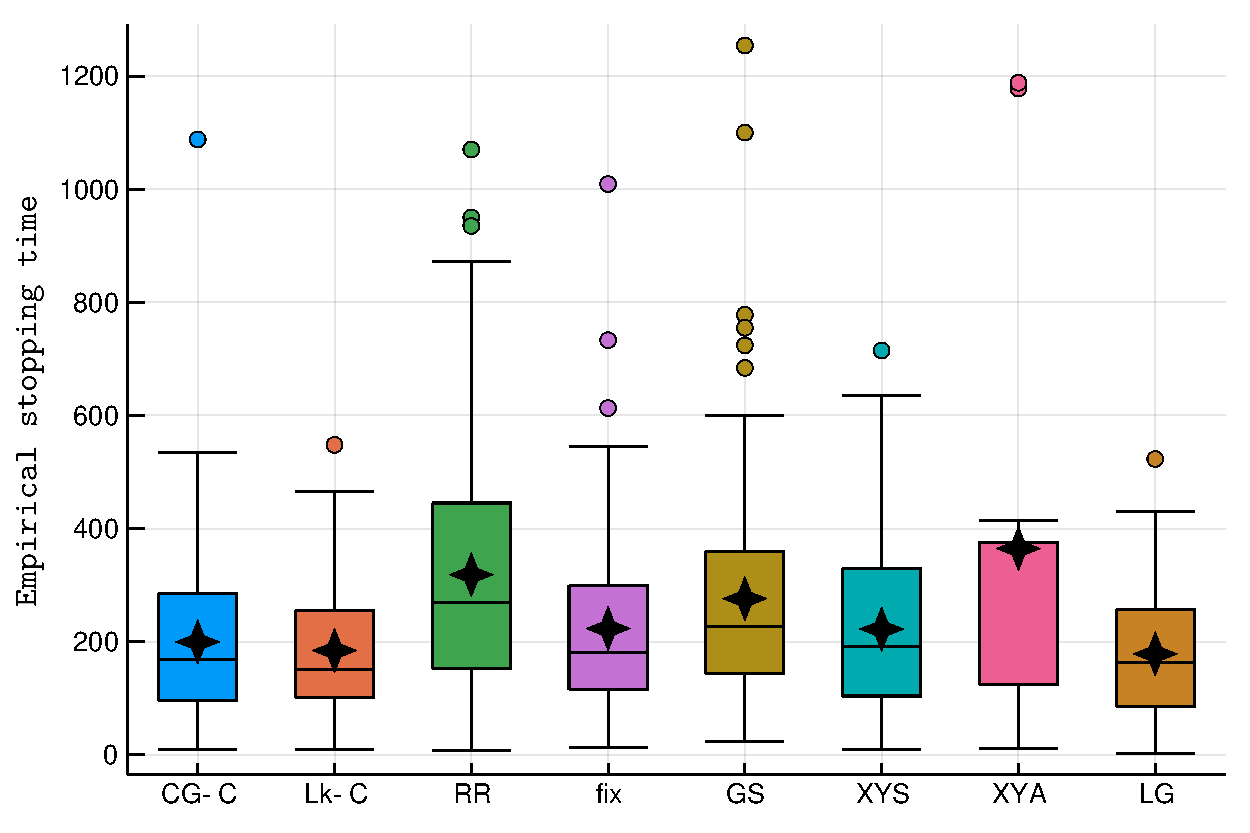
\includegraphics[clip, width= 0.33\textwidth]{Chapter4/img/bai_sin_0-1}
 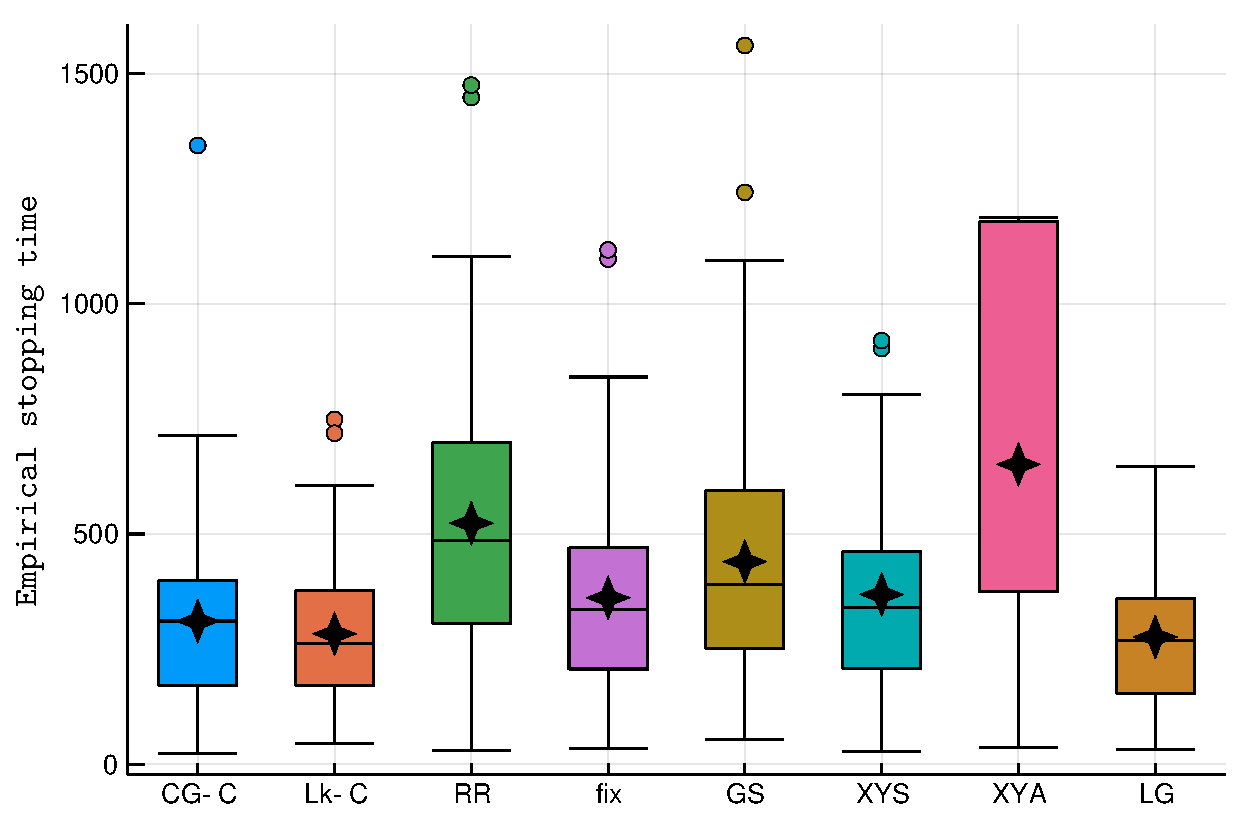
\includegraphics[clip, width= 0.33\textwidth]{Chapter4/img/bai_sin_0-01}
 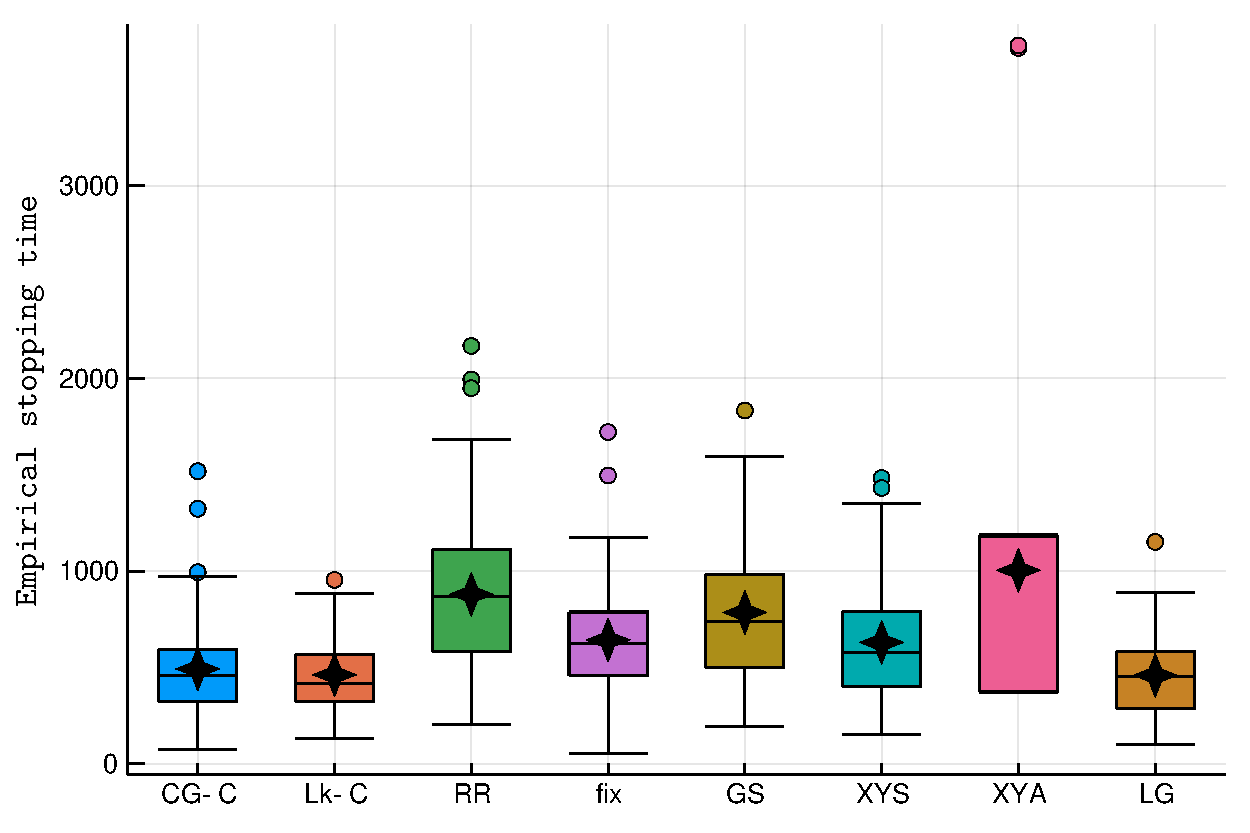
\includegraphics[clip, width= 0.33\textwidth]{Chapter4/img/bai_sin_0-0001}
 \caption{Sample complexity of different linear BAI sampling rules over the usual counter-example with $\delta=0.1, 0.01, 0.0001$ respectively. CG = \LGC,  Lk = \LG, RR = uniform sampling, fix = tracking the fixed weights, GS = \XYS with $\gopt$-allocation, XYS = \XYS with $\xyopt$-allocation, LG = \LGapE. The mean stopping time is represented by a black cross.}
 \label{fig:sample_complexity_1}
\end{figure}

For the second instance, we consider 20 arms randomly generated from the unit sphere $\mathbb{S}^{d-1}\eqdef\{a\in\R^d; \normm{a}_2=1\}$. We choose the two closest arms $a, a'$ and we set $\theta = a + 0.01(a'-a)$ so that a is the best arm. This setting has already been considered by~\citet{tao2018alba}. We report the same box plots over 100 replications as before with increasing dimension in Fig.~\ref{fig:sample_complexity_2}. More precisely, we set $d=6, 8, 10, 12$ respectively, and always keep a same $\delta = 0.01$. Our algorithms consistently show strong performances compared to other algorithms apart from \LGapE.
%Moreover, we can see that in these random examples, \LGC works better than the non-confexified one, and is even competitive compared to \LGapE.


\begin{figure}[ht]
 \centering
 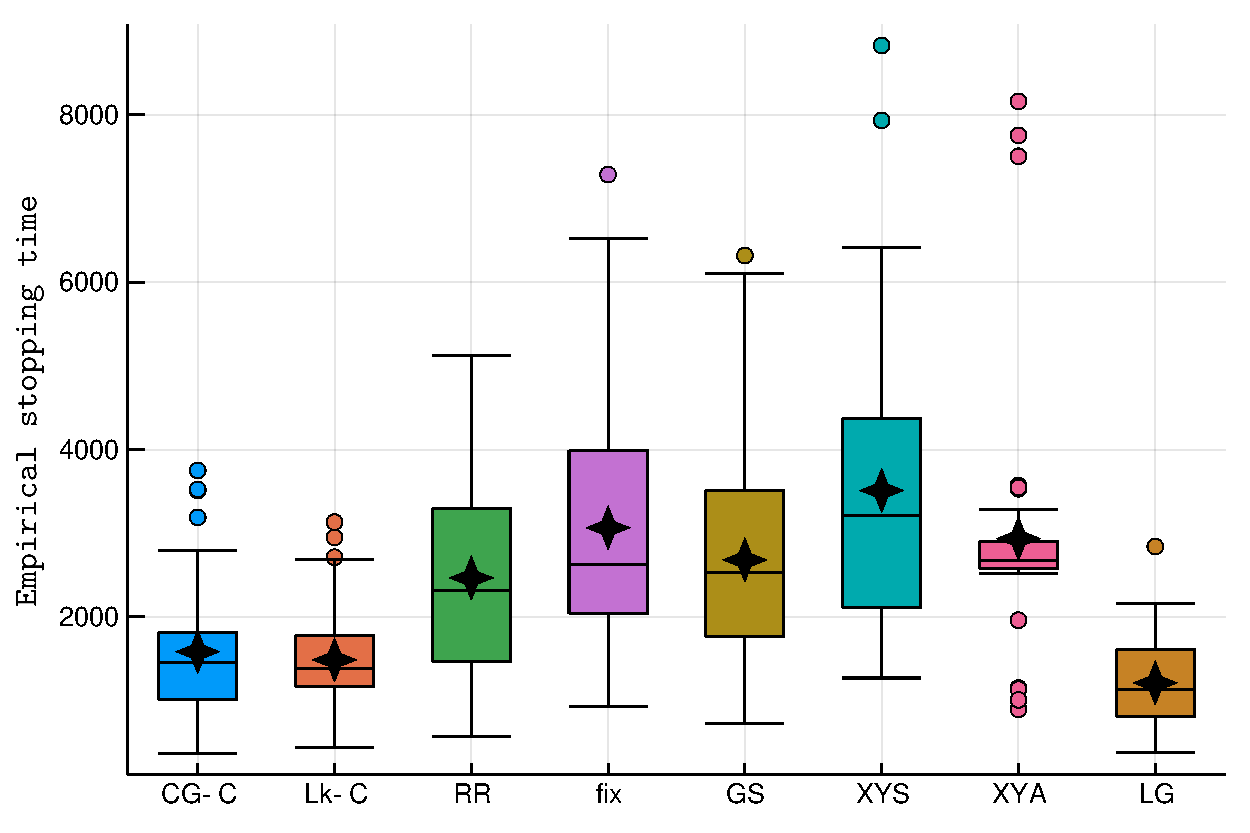
\includegraphics[clip, width= 0.33\textwidth]{Chapter4/img/bai_dim_6}
 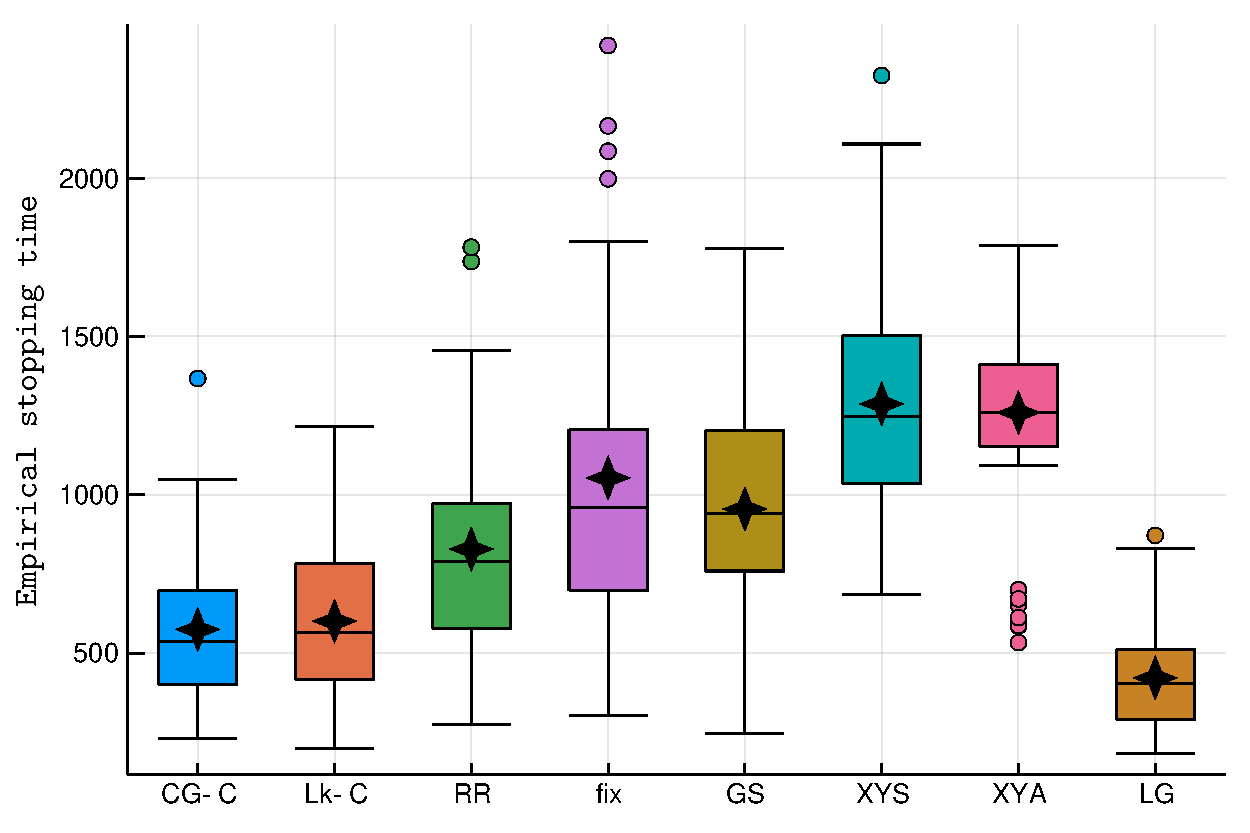
\includegraphics[clip, width= 0.33\textwidth]{Chapter4/img/bai_dim_8}
 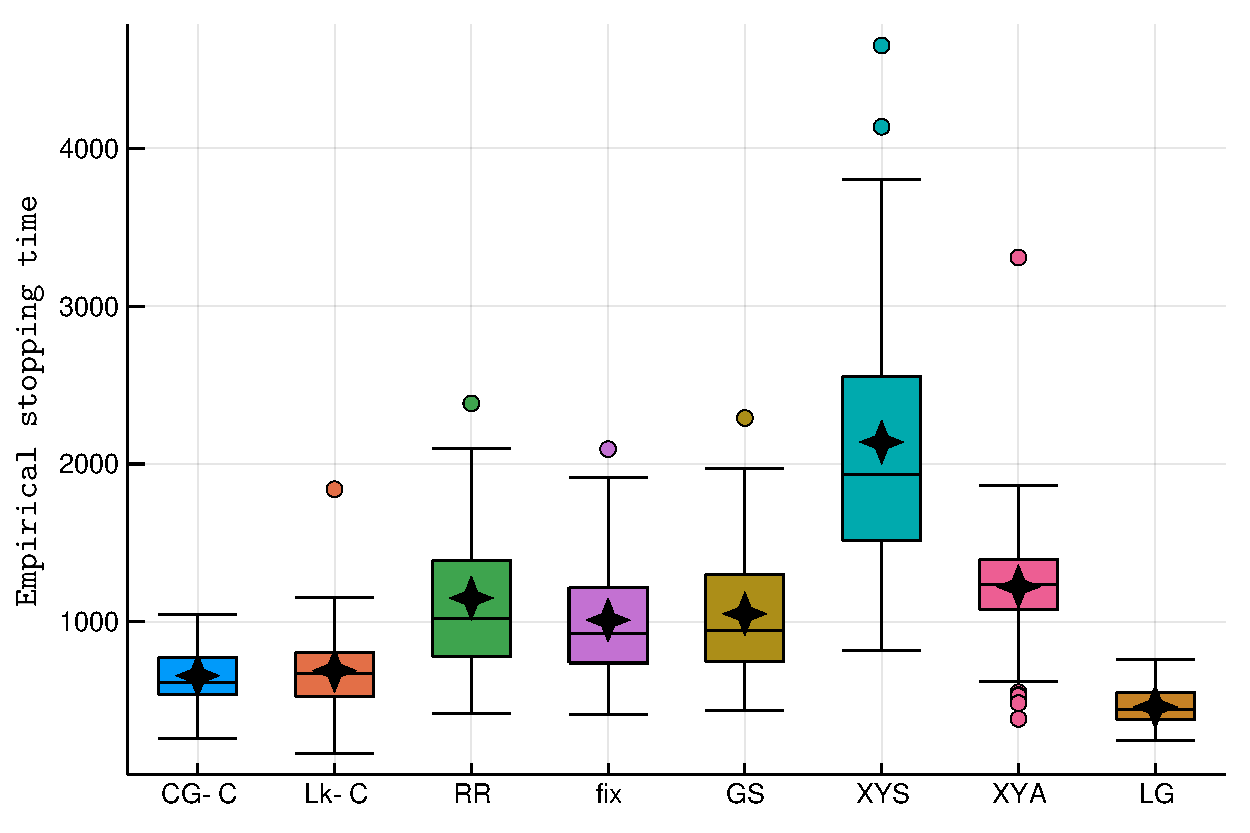
\includegraphics[clip, width= 0.33\textwidth]{Chapter4/img/bai_dim_10}
 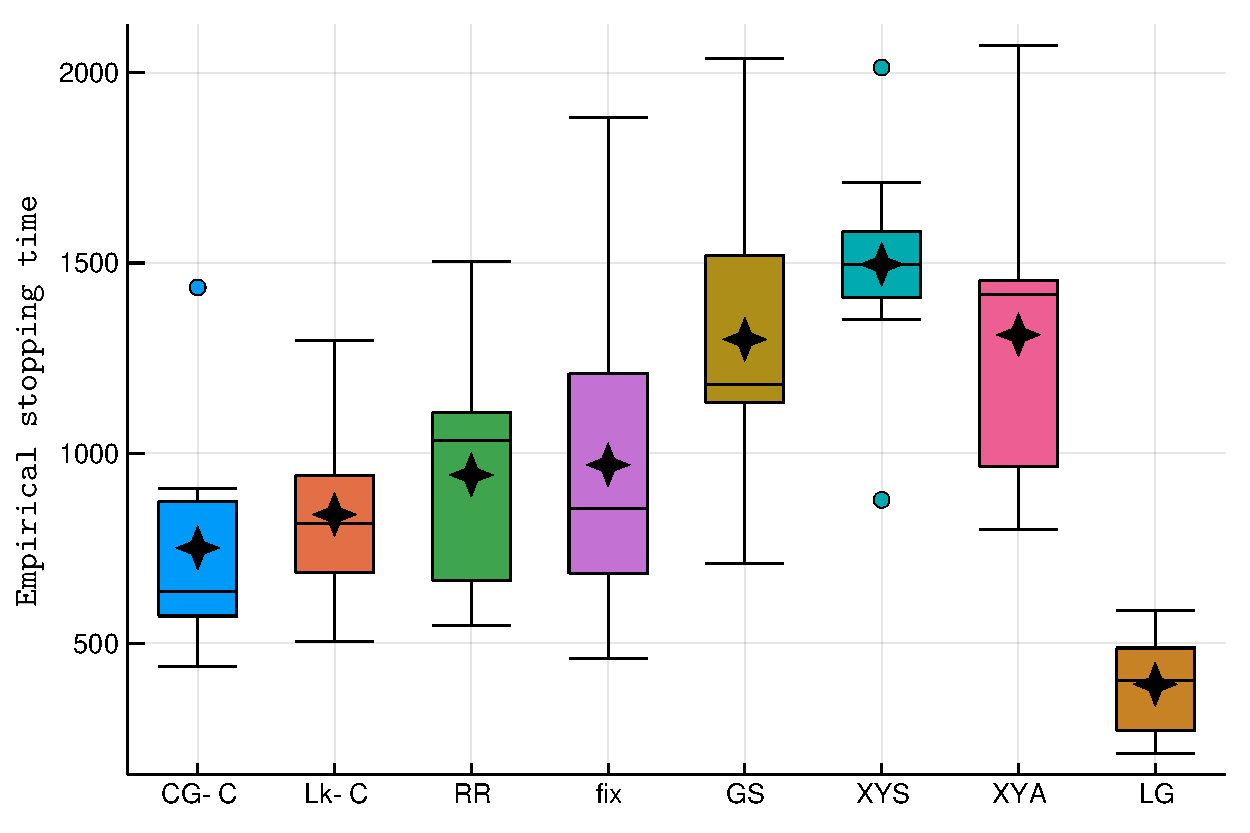
\includegraphics[clip, width= 0.34\textwidth]{Chapter4/img/bai_dim_12}
 \caption{Sample complexity of different linear BAI sampling rules over random unit sphere vectors with $d=6, 8, 10, 12$ from left to right.}
 \label{fig:sample_complexity_2}
\end{figure}

%We stress that although the main focus of this chapter is theoretical, with algorithms that are asymptotically optimal, our methods are also competitive with earlier algorithms experimentally.

